\chapter{Results}
\label{ch:results}

This chapter presents the quantitative results of the experimental campaign in the following order: Section~\ref{sec:covariance_results} reports continual-learning metrics for the covariance estimators and mixture-of-Gaussian variants; Section~\ref{sec:df_results} covers the generative--discriminative re-ranking strategies; Section~\ref{sec:backbone_results} ablates the choice of feature extractor; Section~\ref{sec:incremental_update} presents the sample efficiency and incremental class-inclusion curves; Section~\ref{sec:pca_results} reports the PCA spectral decay of the DINOv2 embeddings; Section~\ref{sec:interclass_results} characterises inter-class separability via pairwise KL divergence; Section~\ref{sec:gaussianity_results_combined} consolidates the marginal and multivariate Gaussianity tests; and Section~\ref{sec:calibration_results_section} reports the probabilistic confidence and calibration metrics. All interpretation is deferred to Chapter~\ref{ch:analysis}.

For every benchmark we report the average accuracy after the last task, $A_{T}$, and the forgetting score $F_{T}$ as defined in Chapter~\ref{methodolohy}. Whenever possible we report mean and variance over three independent runs (different task-order seeds). Since the proposed Gaussian classifiers maintain only sufficient statistics $(\boldsymbol{\mu}_c, \Sigma_c)$ and do not involve parameter optimisation during incremental updates, the resulting classifier is independent of the specific class-presentation order; this explains the $\pm 0.00$ standard deviation reported for our methods throughout. State-of-the-art prompt-based competitors are reproduced from the published values reported in their respective papers. Methods proposed in this thesis are highlighted in grey. The best result per column is shown in bold.

A further structural property deserves attention before examining the tables. The proposed framework does not exhibit forgetting in the conventional sense of parameter overwriting: previously learned class statistics are never modified when new classes are introduced. The forgetting values reported here therefore reflect \emph{statistical interference}---the increased difficulty of the multi-class decision as the number of competing class prototypes grows---rather than degradation of previously learned representations.

\section{Covariance Estimation and Mixtures of Gaussians}
\label{sec:covariance_results}

Table~\ref{tab:combined_benchmarks} reports the average accuracy and the forgetting score for every covariance estimator (diagonal, full, hybrid, Ledoit--Wolf identity/diagonal target~\cite{Ledoit2004}, OAS~\cite{Chen2010}) and for the mixture-of-Gaussian variants MOG-$k$ with $k\in\{2,4\}$ components and three sub-variants (\textit{D}, \textit{F}, \textit{H} for diagonal, full and hybrid covariance respectively). The first block compares our methods against prompt-based state-of-the-art baselines reproduced from the literature. Table~\ref{tab:split_joint} reports the same family on the 30-task Joint stream.

\begin{table}[htb]
	\centering
	\caption{Continual-learning performance on the three 10-task benchmarks. $A_{10}$ and $F_{10}$ are reported in percentage points.}
	\label{tab:combined_benchmarks}
	\scriptsize
	\begin{tabularx}{\textwidth}{lXXXXXX}
		\toprule
		\textbf{Method} & \multicolumn{2}{c}{\textbf{Split CIFAR-100}} & \multicolumn{2}{c}{\textbf{Split ImageNet-R}} & \multicolumn{2}{c}{\textbf{Split Caltech-256}} \\
		\cmidrule(lr){2-3} \cmidrule(lr){4-5} \cmidrule(lr){6-7}
		& \multicolumn{1}{c}{$A_{10} (\uparrow)$} & \multicolumn{1}{c}{$F_{10} (\downarrow)$} & \multicolumn{1}{c}{$A_{10} (\uparrow)$} & \multicolumn{1}{c}{$F_{10} (\downarrow)$} & \multicolumn{1}{c}{$A_{10} (\uparrow)$} & \multicolumn{1}{c}{$F_{10} (\downarrow)$} \\
		\midrule
		L2P             & $83.86 \pm 1.17$ & $7.35 \pm 0.39$ & $61.57 \pm 0.40$ & $9.73 \pm 0.42$ & $92.11 \pm 0.32$ & $2.94 \pm 0.26$ \\
		DualPrompt      & $86.51 \pm 0.49$ & $5.16 \pm 0.20$ & $68.13 \pm 0.52$ & $4.68 \pm 0.18$ & $92.50 \pm 0.16$ & $2.50 \pm 0.16$ \\
		DualPrompt-PGP  & $86.92 \pm 0.05$ & $5.35 \pm 0.19$ & $69.34 \pm 0.05$ & $4.53 \pm 0.04$ & --- & --- \\
		CODA-Prompt     & $87.00 \pm 0.38$ & $4.78 \pm 0.24$ & $74.24 \pm 0.56$ & $4.92 \pm 0.21$ & --- & --- \\
		CPrompt         & $87.83 \pm 0.37$ & $4.88 \pm 0.79$ & $76.71 \pm 0.61$ & $4.66 \pm 0.93$ & --- & --- \\
		ConvPrompt      & $88.87 \pm 0.33$ & $4.75 \pm 0.15$ & $77.86 \pm 0.25$ & $4.33 \pm 0.24$ & --- & --- \\
		RainbowPrompt   & $\mathbf{89.86 \pm 0.11}$ & $\mathbf{3.44 \pm 0.26}$ & $79.09 \pm 0.13$ & $3.90 \pm 0.23$ & --- & --- \\
		APT             & $88.88 \pm 0.65$ & $3.47 \pm 0.55$ & $\mathbf{79.40 \pm 0.47}$ & $4.38 \pm 0.46$ & --- & --- \\
		\midrule
		\rowcolor{gray!15} Diag-Cov (ours)         & $86.07 \pm 0.00$ & $4.30 \pm 0.12$ & $77.12 \pm 0.00$ & $7.44 \pm 0.17$ & $90.06 \pm 0.00$ & $\mathbf{1.69 \pm 0.36}$ \\
		\rowcolor{gray!15} Full-Cov (ours)         & $88.48 \pm 0.00$ & $4.18 \pm 0.00$ & $75.08 \pm 0.00$ & $5.07 \pm 0.03$ & $90.01 \pm 0.01$ & $2.16 \pm 0.05$ \\
		\rowcolor{gray!15} Hybrid-Cov (ours)       & $88.49 \pm 0.00$ & $4.18 \pm 0.00$ & $75.12 \pm 0.00$ & $5.03 \pm 0.04$ & $94.36 \pm 0.00$ & $2.09 \pm 0.08$ \\
		\rowcolor{gray!15} Shared-Diag-Cov (ours)  & $86.54 \pm 0.00$ & $4.61 \pm 0.10$ & $75.12 \pm 0.01$ & $4.80 \pm 0.24$ & $93.00 \pm 0.00$ & $2.00 \pm 0.11$ \\
		\rowcolor{gray!15} Shared-Full-Cov (ours)  & $88.56 \pm 0.00$ & $3.76 \pm 0.11$ & $77.06 \pm 0.01$ & $\mathbf{3.97 \pm 0.30}$ & $93.54 \pm 0.00$ & $2.05 \pm 0.29$ \\
		\rowcolor{gray!15} MOG2-D (ours)           & $86.96 \pm 0.00$ & $4.24 \pm 0.02$ & $70.15 \pm 0.00$ & $4.93 \pm 0.02$ & $91.41 \pm 0.00$ & $1.67 \pm 0.30$ \\
		\rowcolor{gray!15} MOG2-F (ours)           & $85.01 \pm 0.00$ & $5.13 \pm 0.17$ & $73.42 \pm 0.00$ & $5.49 \pm 0.26$ & $93.95 \pm 0.00$ & $2.14 \pm 0.11$ \\
		\rowcolor{gray!15} MOG2-H (ours)           & $84.68 \pm 0.00$ & $5.26 \pm 0.22$ & $73.52 \pm 0.00$ & $5.47 \pm 0.23$ & $93.93 \pm 0.00$ & $2.13 \pm 0.10$ \\
		\rowcolor{gray!15} MOG4-D (ours)           & $87.80 \pm 0.00$ & $4.02 \pm 0.06$ & $72.52 \pm 0.01$ & $5.06 \pm 0.15$ & $91.12 \pm 0.00$ & $1.63 \pm 0.31$ \\
		\rowcolor{gray!15} MOG4-F (ours)           & $88.87 \pm 0.00$ & $3.99 \pm 0.00$ & $75.07 \pm 0.00$ & $5.07 \pm 0.05$ & $\mathbf{94.39 \pm 0.00}$ & $2.12 \pm 0.08$ \\
		\rowcolor{gray!15} MOG4-H (ours)           & $88.88 \pm 0.00$ & $4.04 \pm 0.00$ & $75.01 \pm 0.00$ & $5.12 \pm 0.04$ & $94.36 \pm 0.00$ & $2.09 \pm 0.08$ \\
		\rowcolor{gray!15} OAS (ours)              & $84.38 \pm 0.00$ & $3.90 \pm 0.07$ & $71.47 \pm 0.00$ & $4.57 \pm 0.29$ & $86.70 \pm 0.00$ & $1.90 \pm 1.77$ \\
		\rowcolor{gray!15} LW-I (ours)             & $84.78 \pm 0.00$ & $3.93 \pm 0.09$ & $71.91 \pm 0.00$ & $4.54 \pm 0.43$ & $89.89 \pm 0.00$ & $1.50 \pm 0.08$ \\
		\rowcolor{gray!15} LW-D (ours)             & $82.85 \pm 0.00$ & $3.94 \pm 0.28$ & $70.35 \pm 0.00$ & $4.62 \pm 0.95$ & $90.04 \pm 0.00$ & $1.66 \pm 0.30$ \\
		\bottomrule
	\end{tabularx}
\end{table}

\begin{table}[htbp]
	\centering
	\caption{Performance on the long-horizon \textbf{Split Joint Datasets} benchmark (30 tasks aggregated from CIFAR-100, ImageNet-R and Caltech-256). $A_{30}$ and $F_{30}$ are reported in percentage points.}
	\label{tab:split_joint}
	\scriptsize
	\newcolumntype{Y}{>{\centering\arraybackslash}X}
	\begin{tabularx}{0.6\textwidth}{lYY}
		\toprule
		\textbf{Method} & \multicolumn{2}{c}{\textbf{Split Joint Datasets}} \\
		\cmidrule(lr){2-3}
		& $A_{30} (\uparrow)$ & $F_{30} (\downarrow)$ \\
		\midrule
		Diag-Cov        & $78.32 \pm 0.21$ & $6.05 \pm 0.12$ \\
		Full-Cov        & $78.65 \pm 0.00$ & $4.69 \pm 0.02$ \\
		Hybrid-Cov      & $\mathbf{83.42 \pm 0.00}$ & $\mathbf{3.86 \pm 0.04}$ \\
		Shared-Full-Cov & $80.77 \pm 0.00$ & $4.47 \pm 0.08$ \\
		Shared-Diag-Cov & $79.52 \pm 0.00$ & $4.95 \pm 0.18$ \\
		MOG2-D          & $73.91 \pm 0.02$ & $5.69 \pm 0.02$ \\
		MOG2-F          & $78.41 \pm 0.02$ & $5.85 \pm 0.04$ \\
		MOG2-H          & $80.27 \pm 0.02$ & $5.04 \pm 0.04$ \\
		MOG4-D          & $80.28 \pm 0.01$ & $4.67 \pm 0.00$ \\
		MOG4-F          & $59.68 \pm 0.25$ & $5.88 \pm 0.16$ \\
		MOG4-H          & $58.01 \pm 0.30$ & $5.97 \pm 0.09$ \\
		OAS             & $77.46 \pm 0.00$ & $4.60 \pm 0.10$ \\
		LW-I            & $76.41 \pm 0.01$ & $5.83 \pm 0.31$ \\
		LW-D            & $77.42 \pm 0.02$ & $5.41 \pm 0.38$ \\
		\bottomrule
	\end{tabularx}
\end{table}

\section{Generative--Discriminative Fusion and Re-ranking Strategies}
\label{sec:df_results}

Tables~\ref{tab:hybrid_cifar}--\ref{tab:hybrid_joint} report the effect of the ten re-ranking and fusion strategies introduced in Chapter~\ref{methodolohy}, paired with both the diagonal and the full covariance branch on every benchmark. The rows of each table are grouped according to the recommendation taxonomy derived in Section~\ref{sec:an:taxonomy}: the upper block lists the \emph{recommended} strategies (SoftTaskFus, TaskMeanShr, Top5-CosRR, OptFusion-MM, TempScale), the middle block lists the \emph{non-recommended (brittle)} strategies (HardGate, Top5-TaskRR, TopK-TaskFilt) and the lower block lists the \emph{marginal} strategies (HardGate-LDA, SoftGate-LDA), with a horizontal rule separating the three groups.

\begin{table}[htbp]
	\centering
	\caption{Generative--Discriminative Re-ranking Strategies on \textbf{Split CIFAR-100}.}
	\label{tab:hybrid_cifar}
	\scriptsize
	\begin{tabular}{l cccc}
		\toprule
		\textbf{Strategy} & \multicolumn{2}{c}{\textbf{Diag-Cov}} & \multicolumn{2}{c}{\textbf{Full-Cov}} \\
		\cmidrule(lr){2-3} \cmidrule(lr){4-5}
		& $A_{10} (\uparrow)$ & $F_{10} (\downarrow)$ & $A_{10} (\uparrow)$ & $F_{10} (\downarrow)$ \\
		\midrule

		SoftTaskFus    & $86.16 \pm 0.00$ & $4.41 \pm 0.05$ & $88.52 \pm 0.00$ & $4.18 \pm 0.00$ \\
		TaskMeanShr    & $86.08 \pm 0.00$ & $4.29 \pm 0.12$ & $88.48 \pm 0.00$ & $4.17 \pm 0.00$ \\
		Top5-CosRR     & $86.59 \pm 0.00$ & $4.92 \pm 0.12$ & $87.05 \pm 0.00$ & $4.91 \pm 0.10$ \\
		OptFusion-MM   & $\mathbf{87.04 \pm 0.00}$ & $4.82 \pm 0.07$ & $\mathbf{89.23 \pm 0.00}$ & $4.17 \pm 0.03$ \\
		TempScale      & $86.24 \pm 0.00$ & $\mathbf{4.22 \pm 0.10}$ & $88.86 \pm 0.00$ & $\mathbf{4.05 \pm 0.00}$ \\
		\midrule
		HardGate       & $73.60 \pm 0.88$ & $9.82 \pm 0.17$ & $86.56 \pm 0.00$ & $4.83 \pm 0.48$ \\
		Top5-TaskRR    & $75.02 \pm 1.09$ & $8.80 \pm 0.53$ & $86.71 \pm 0.01$ & $4.73 \pm 0.46$ \\
		TopK-TaskFilt  & $83.90 \pm 0.15$ & $6.30 \pm 0.34$ & $88.51 \pm 0.01$ & $4.25 \pm 0.02$ \\
		\midrule
		HardGate-LDA   & $73.83 \pm 0.77$ & $9.93 \pm 0.14$ & $86.97 \pm 0.02$ & $4.89 \pm 0.53$ \\
		SoftGate-LDA   & $81.07 \pm 0.07$ & $6.79 \pm 0.14$ & $87.19 \pm 0.03$ & $4.79 \pm 0.62$ \\
		\bottomrule
	\end{tabular}
\end{table}

\begin{table}[htbp]
	\centering
	\caption{Generative--Discriminative Re-ranking Strategies on \textbf{Split ImageNet-R}.}
	\label{tab:hybrid_imagenet}
	\scriptsize
	\begin{tabular}{l cccc}
		\toprule
		\textbf{Strategy} & \multicolumn{2}{c}{\textbf{Diag-Cov}} & \multicolumn{2}{c}{\textbf{Full-Cov}} \\
		\cmidrule(lr){2-3} \cmidrule(lr){4-5}
		& $A_{10} (\uparrow)$ & $F_{10} (\downarrow)$ & $A_{10} (\uparrow)$ & $F_{10} (\downarrow)$ \\
		\midrule

		SoftTaskFus    & $75.04 \pm 0.02$ & $\mathbf{4.30 \pm 0.61}$ & $63.11 \pm 0.00$ & $6.72 \pm 9.39$ \\
		TaskMeanShr    & $75.21 \pm 0.00$ & $4.37 \pm 0.68$  & $62.80 \pm 0.00$ & $6.85 \pm 9.57$ \\
		Top5-CosRR     & $\mathbf{76.20 \pm 0.00}$ & $5.01 \pm 0.36$  & $73.63 \pm 0.01$ & $6.31 \pm 2.45$ \\
		OptFusion-MM   & $76.65 \pm 0.00$ & $5.38 \pm 0.42$  & $\mathbf{77.00 \pm 0.00}$ & $\mathbf{4.94 \pm 1.23}$ \\
		TempScale      & $74.68 \pm 0.00$ & $4.87 \pm 0.52$  & $67.17 \pm 0.00$ & $6.00 \pm 6.82$ \\
		\midrule
		HardGate       & $53.95 \pm 0.59$ & $11.65 \pm 0.83$ & $69.78 \pm 0.09$ & $4.54 \pm 2.45$ \\
		Top5-TaskRR    & $56.49 \pm 0.52$ & $9.82 \pm 1.23$  & $69.53 \pm 0.11$ & $4.64 \pm 2.75$ \\
		TopK-TaskFilt  & $68.65 \pm 0.30$ & $7.79 \pm 0.35$  & $65.46 \pm 1.36$ & $5.24 \pm 8.95$ \\
		\midrule
		HardGate-LDA   & $54.14 \pm 0.54$ & $11.88 \pm 0.70$ & $73.70 \pm 0.09$ & $6.08 \pm 3.86$ \\
		SoftGate-LDA   & $59.90 \pm 0.25$ & $9.78 \pm 2.10$  & $73.72 \pm 0.12$ & $6.15 \pm 5.84$ \\
		\bottomrule
	\end{tabular}
\end{table}

\begin{table}[htbp]
	\centering
	\caption{Generative--Discriminative Re-ranking Strategies on \textbf{Split Caltech-256}.}
	\label{tab:hybrid_caltech}
	\scriptsize
	\begin{tabular}{l cccc}
		\toprule
		\textbf{Strategy} & \multicolumn{2}{c}{\textbf{Diag-Cov}} & \multicolumn{2}{c}{\textbf{Full-Cov}} \\
		\cmidrule(lr){2-3} \cmidrule(lr){4-5}
		& $A_{10} (\uparrow)$ & $F_{10} (\downarrow)$ & $A_{10} (\uparrow)$ & $F_{10} (\downarrow)$ \\
		\midrule

		SoftTaskFus    & $90.87 \pm 0.00$ & $1.60 \pm 0.35$ & $\mathbf{95.03 \pm 0.00}$ & $\mathbf{1.68 \pm 0.03}$ \\
		TaskMeanShr    & $86.08 \pm 0.00$ & $4.29 \pm 0.12$ & $94.73 \pm 0.00$ & $1.84 \pm 0.02$ \\
		Top5-CosRR     & $91.99 \pm 0.00$ & $2.44 \pm 0.13$ & $94.03 \pm 0.00$ & $2.25 \pm 0.01$ \\
		OptFusion-MM   & $\mathbf{93.96 \pm 0.00}$ & $2.28 \pm 0.01$ & $94.78 \pm 0.00$ & $1.94 \pm 0.04$ \\
		TempScale      & $89.68 \pm 0.00$ & $1.86 \pm 0.55$ & $94.40 \pm 0.00$ & $1.89 \pm 0.05$ \\
		\midrule
		HardGate       & $80.36 \pm 0.11$ & $5.48 \pm 0.16$ & $92.77 \pm 0.04$ & $2.34 \pm 0.09$ \\
		Top5-TaskRR    & $90.53 \pm 0.00$ & $1.53 \pm 0.04$ & $92.94 \pm 0.05$ & $2.25 \pm 0.10$ \\
		TopK-TaskFilt  & $88.06 \pm 0.06$ & $3.20 \pm 0.11$ & $94.58 \pm 0.01$ & $1.99 \pm 0.02$ \\
		\midrule
		HardGate-LDA   & $82.10 \pm 0.77$ & $5.59 \pm 0.36$ & $92.57 \pm 0.01$ & $1.75 \pm 0.10$ \\
		SoftGate-LDA   & $87.64 \pm 0.02$ & $3.40 \pm 1.41$ & $92.26 \pm 0.05$ & $1.73 \pm 0.06$ \\
		\bottomrule
	\end{tabular}
\end{table}

\begin{table}[htbp]
	\centering
	\caption{Generative--Discriminative Re-ranking Strategies on \textbf{Split Joint Datasets} (30 tasks).}
	\label{tab:hybrid_joint}
	\scriptsize
	\begin{tabular}{l cccc}
		\toprule
		\textbf{Strategy} & \multicolumn{2}{c}{\textbf{Diag-Cov}} & \multicolumn{2}{c}{\textbf{Full-Cov}} \\
		\cmidrule(lr){2-3} \cmidrule(lr){4-5}
		& $A_{30} (\uparrow)$ & $F_{30} (\downarrow)$ & $A_{30} (\uparrow)$ & $F_{30} (\downarrow)$ \\
		\midrule

		SoftTaskFus    & $78.86 \pm 0.00$ & $\mathbf{4.97 \pm 0.09}$ & $52.50 \pm 0.00$ & $8.44 \pm 2.67$ \\
		TaskMeanShr    & $78.13 \pm 0.00$ & $5.20 \pm 0.13$ & $52.14 \pm 0.00$ & $8.61 \pm 2.87$ \\
		Top5-CosRR     & $78.92 \pm 0.00$ & $5.41 \pm 0.08$ & $63.61 \pm 0.00$ & $7.08 \pm 1.29$ \\
		OptFusion-MM   & $\mathbf{79.08 \pm 0.00}$ & $5.67 \pm 0.08$ & $\mathbf{81.94 \pm 0.00}$ & $4.89 \pm 0.02$ \\
		TempScale      & $78.79 \pm 0.00$ & $5.26 \pm 0.09$ & $69.67 \pm 0.00$ & $6.93 \pm 1.25$ \\
		\midrule
		HardGate       & $66.11 \pm 0.00$ & $9.70 \pm 0.21$ & $53.16 \pm 0.00$ & $5.53 \pm 1.98$ \\
		Top5-TaskRR    & $68.59 \pm 0.00$ & $7.80 \pm 0.12$ & $52.03 \pm 0.00$ & $5.83 \pm 2.46$ \\
		TopK-TaskFilt  & $75.41 \pm 0.00$ & $6.45 \pm 0.03$ & $47.61 \pm 0.00$ & $7.48 \pm 3.87$ \\
		\midrule
		HardGate-LDA   & $66.52 \pm 0.00$ & $8.66 \pm 0.22$ & $53.02 \pm 0.00$ & $4.75 \pm 0.46$ \\
		SoftGate-LDA   & $68.25 \pm 0.00$ & $8.94 \pm 4.00$ & $52.07 \pm 0.00$ & $\mathbf{4.81 \pm 0.62}$ \\
		\bottomrule
	\end{tabular}
\end{table}

\section{Backbones Comparison}
\label{sec:backbone_results}

Table~\ref{tab:multi_backbone_results} reports the two best closed-form estimators (Diag-Cov and Full-Cov) when paired with three vision backbones: DINOv2~\cite{oquab2024dinov} (the default of this work), ViT-base patch-16/224 and ViT-medium patch-16/224, both supplied by the \texttt{timm} library~\cite{rw2019timm}.

\begin{table}[htbp]
	\centering
	\caption{Backbone ablation. The two best closed-form estimators (Diag-Cov and Full-Cov) are evaluated with three vision backbones across all four benchmarks.}
	\label{tab:multi_backbone_results}
	\scriptsize
	\setlength{\tabcolsep}{3.5pt}
	\begin{tabular}{ll cccccccc}
		\toprule
		\textbf{Method} & \textbf{Backbone} & \multicolumn{2}{c}{\textbf{Split CIFAR-100}} & \multicolumn{2}{c}{\textbf{Split ImageNet-R}} & \multicolumn{2}{c}{\textbf{Split Caltech-256}} & \multicolumn{2}{c}{\textbf{Split Joint}} \\
		\cmidrule(lr){3-4} \cmidrule(lr){5-6} \cmidrule(lr){7-8} \cmidrule(lr){9-10}
		& & $A_{10} (\uparrow)$ & $F_{10} (\downarrow)$ & $A_{10} (\uparrow)$ & $F_{10} (\downarrow)$ & $A_{10} (\uparrow)$ & $F_{10} (\downarrow)$ & $A_{30} (\uparrow)$ & $F_{30} (\downarrow)$ \\
		\midrule
		Diag-Cov & DINOv2 & $\mathbf{86.07 \pm 0.00}$ & $4.30 \pm 0.12$ & $\mathbf{77.12 \pm 0.00}$ & $7.44 \pm 0.17$ & $90.06 \pm 0.00$ & $1.69 \pm 0.36$ & $\mathbf{78.32 \pm 0.21}$ & $6.05 \pm 0.12$ \\
		         & ViT-m  & $81.41 \pm 0.00$ & $5.28 \pm 0.13$ & $66.11 \pm 0.00$ & $4.79 \pm 0.14$ & $\mathbf{91.41 \pm 0.00}$ & $\mathbf{1.63 \pm 0.12}$ & $50.63 \pm 1.87$ & $5.42 \pm 0.07$ \\
		         & ViT-b  & $81.03 \pm 0.00$ & $\mathbf{4.57 \pm 0.41}$ & $43.08 \pm 0.00$ & $6.41 \pm 0.19$ & $87.72 \pm 0.00$ & $1.74 \pm 0.50$ & $44.64 \pm 1.43$ & $\mathbf{5.47 \pm 0.08}$ \\
		\midrule
		Full-Cov & DINOv2 & $\mathbf{88.48 \pm 0.00}$ & $\mathbf{4.18 \pm 0.00}$ & $\mathbf{75.08 \pm 0.00}$ & $\mathbf{5.07 \pm 0.03}$ & $90.01 \pm 0.01$ & $2.16 \pm 0.05$ & $\mathbf{78.65 \pm 0.00}$ & $\mathbf{4.69 \pm 0.02}$ \\
		         & ViT-m  & $82.42 \pm 0.00$ & $5.25 \pm 0.01$ & $66.44 \pm 0.00$ & $5.18 \pm 0.27$ & $\mathbf{90.11 \pm 0.00}$ & $\mathbf{1.80 \pm 0.12}$ & $42.10 \pm 0.00$ & $9.39 \pm 1.90$ \\
		         & ViT-b  & $80.40 \pm 0.00$ & $5.38 \pm 0.36$ & $45.72 \pm 0.00$ & $7.16 \pm 0.17$ & $87.13 \pm 0.00$ & $1.92 \pm 0.80$ & $66.51 \pm 0.00$ & $5.47 \pm 0.08$ \\
		\bottomrule
	\end{tabular}
\end{table}

\section{Sample Efficiency and Incremental Class Inclusion}
\label{sec:incremental_update}

Figure~\ref{fig:incremental_class_inclusion} illustrates how the Diag-Cov and Full-Cov class-conditional models behave when samples of a new class arrive progressively. After learning an initial set of nine base classes, an additional class is introduced and its training samples are incorporated in steps of $10\,\%$ of the available data. Two representative target classes per benchmark are reported, chosen to span the dataset's class index range. On Split CIFAR-100 (\textbf{a}), the Diag-Cov classifier reaches a strong plateau already with $10\,\%$ of the samples (reflecting the small number of parameters required to estimate $d=768$ diagonal variances), while Full-Cov improves more gradually and surpasses Diag-Cov once 40--70\,\% of the samples are available. On Split ImageNet-R (\textbf{b}), the limited number of training samples per class (${\sim}40$ after the train/test split for some classes) makes the Full-Cov estimator saturate early at a lower-than-CIFAR ceiling; both estimators improve gradually but the gap between Diag-Cov and Full-Cov stays small. On Split Caltech-256 (\textbf{c}), Full-Cov already dominates from the very first $10\,\%$ slice---reflecting the higher visual variability that benefits more from inter-coordinate correlations---and Diag-Cov tracks the Full-Cov curve at a 1--2 point lower plateau.

\begin{figure}[htbp]
	\centering
	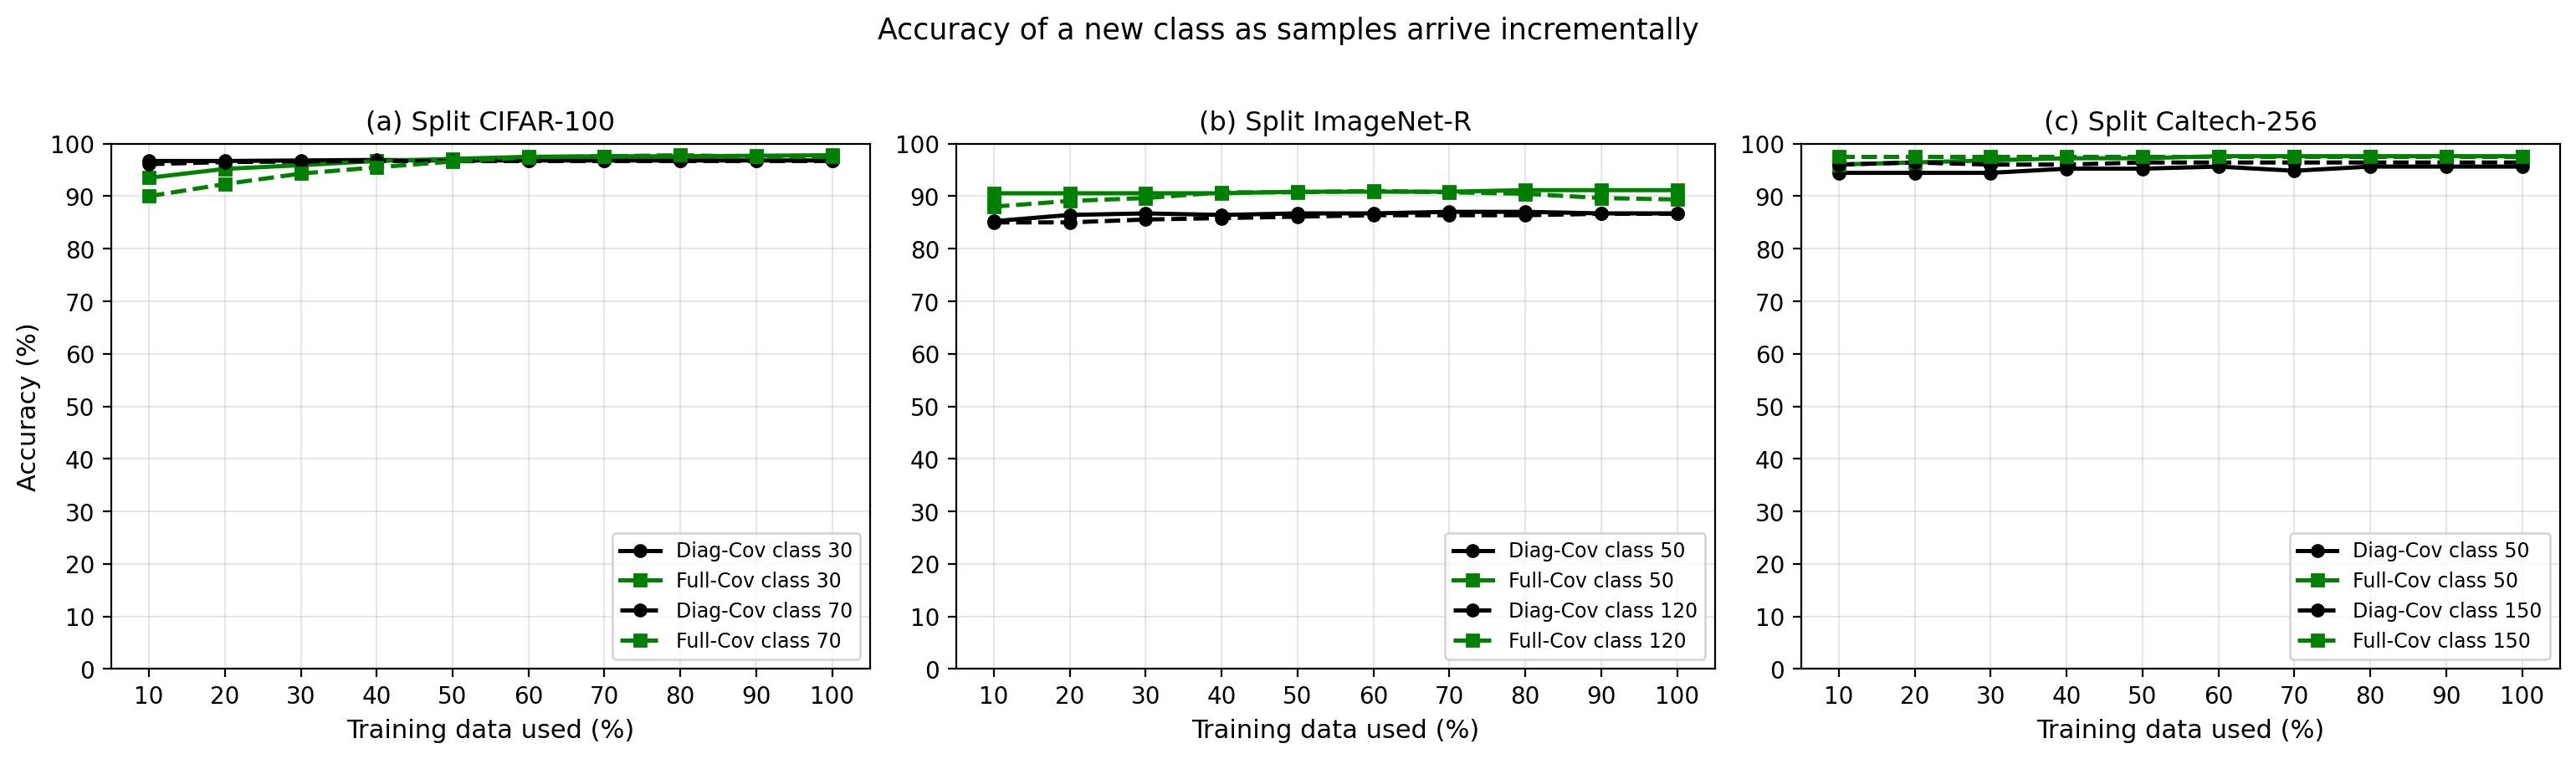
\includegraphics[width=0.97\linewidth]{imagenes/results/incremental_class_inclusion.png}
	\caption{Accuracy of a new class as samples arrive incrementally: (\textbf{a}) Split CIFAR-100, (\textbf{b}) Split ImageNet-R, (\textbf{c}) Split Caltech-256. Two target classes per benchmark are shown. Diag-Cov saturates quickly thanks to its small parameter budget; Full-Cov improves more gradually and eventually surpasses Diag-Cov on CIFAR-100 and Caltech-256, while staying close to it on the data-starved ImageNet-R.}
	\label{fig:incremental_class_inclusion}
\end{figure}

\section{Spectral Analysis of the Embedding Space}
\label{sec:pca_results}

Figure~\ref{fig:pca_eigenvalues} reports the PCA spectral decay of the $\ell_2$-normalised DINOv2 embeddings in percentage-of-variance units. Panel~(a) shows the individual variance contribution of each component: the first component alone explains around $8$--$10\,\%$ of the total variance, and the contribution decays steeply over the first $\sim\!50$ components before levelling off near zero. Panel~(b) shows the cumulative explained variance: roughly $90\,\%$ of the total variance is captured by the leading $100$--$130$ components on all three benchmarks, despite the embedding space being $d=768$-dimensional. The three datasets share remarkably similar spectra across both panels, indicating that the DINOv2 features have a consistent low-intrinsic-dimensionality structure regardless of the image domain.

\begin{figure}[htbp]
	\centering
	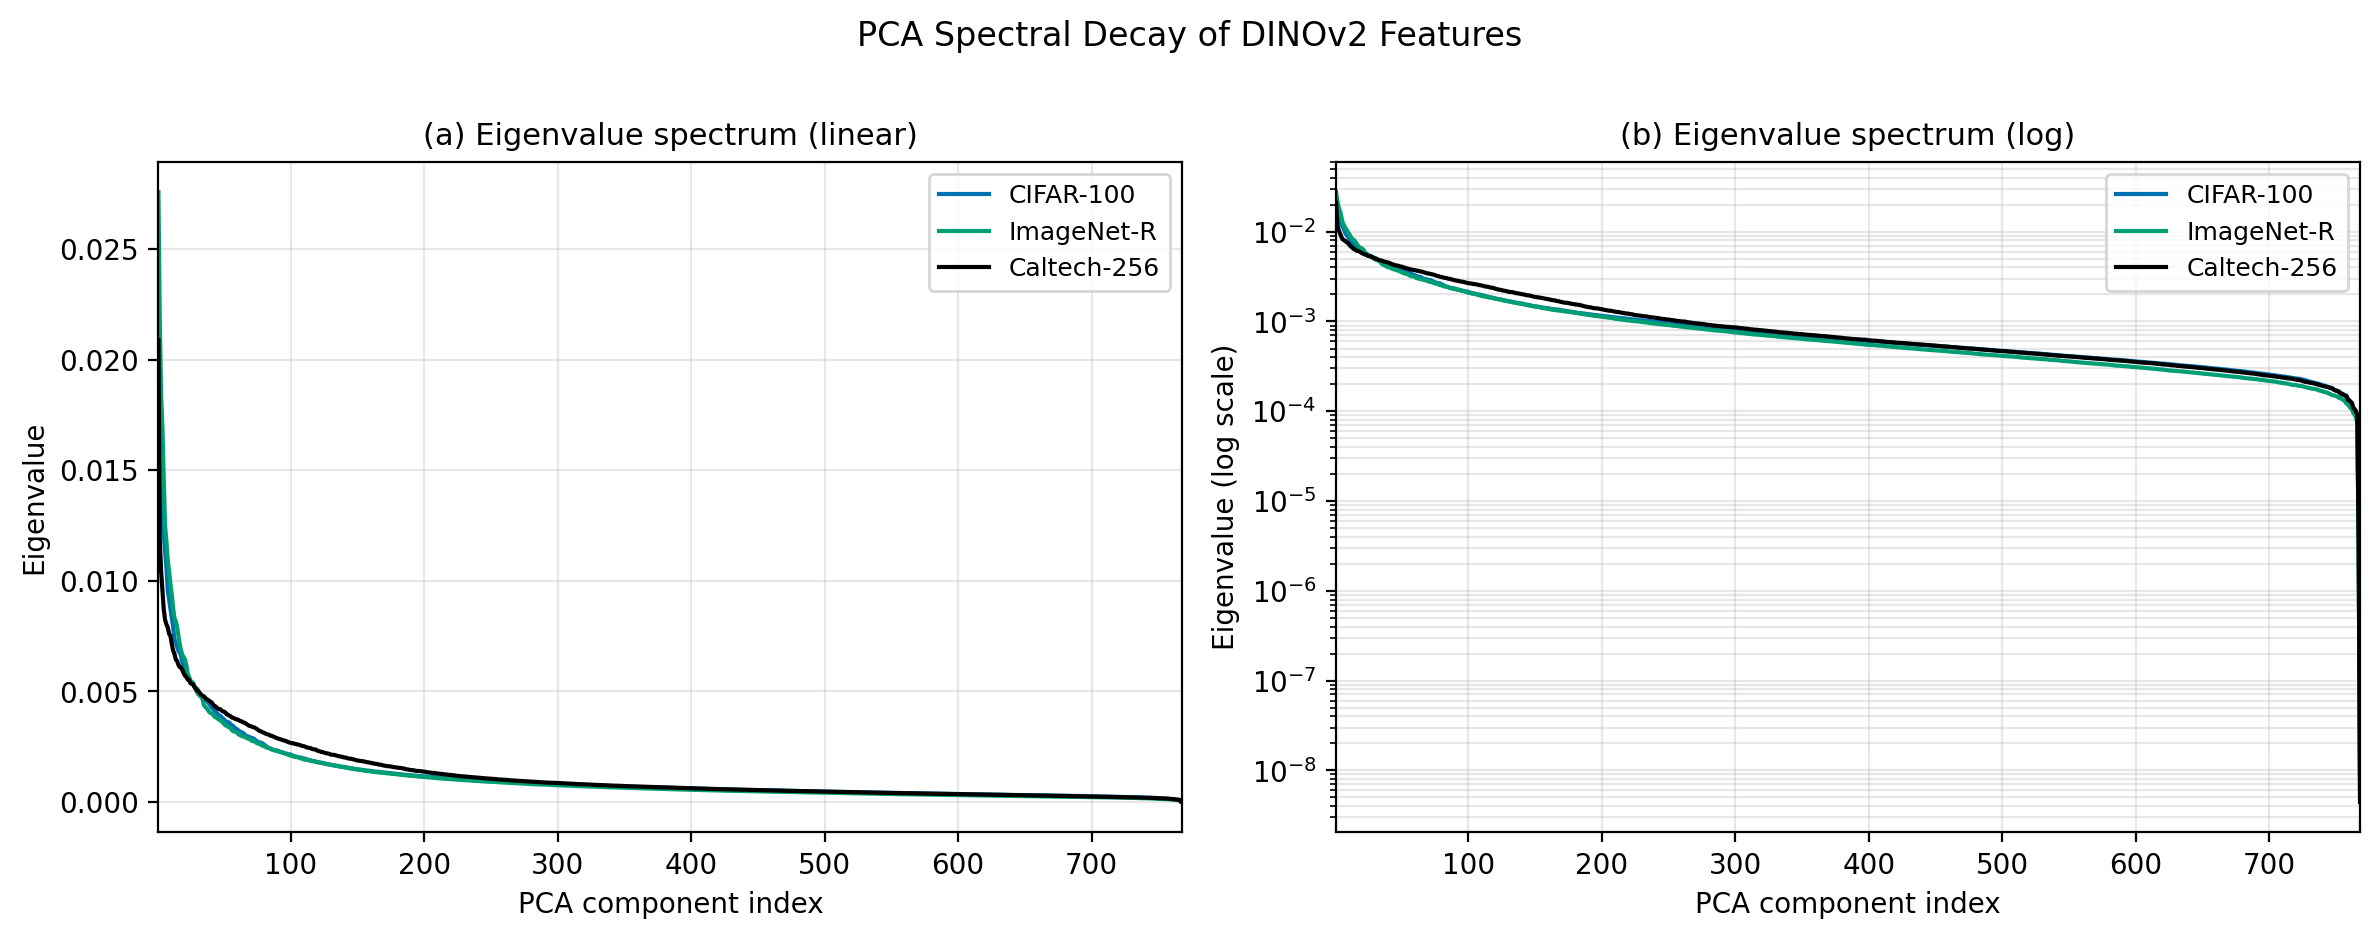
\includegraphics[width=0.97\linewidth]{imagenes/results/pca_eigenvalues.png}
	\caption{PCA spectral decay of the $\ell_2$-normalised DINOv2 features. \textbf{(a)} Individual \% variance explained per component: steep decay over the first $\sim\!50$ components, near-zero contribution thereafter. \textbf{(b)} Cumulative \% variance explained: dashed reference lines mark 50, 80, 90 and 95\,\%; annotated $n$ values show how many components suffice to reach 90\,\% on each dataset. Despite the $d=768$ embedding space, $90\,\%$ of the variance is captured by fewer than 130 components on every benchmark.}
	\label{fig:pca_eigenvalues}
\end{figure}

\section{Inter-Class Pairwise KL Divergence}
\label{sec:interclass_results}

Figure~\ref{fig:kl_divergence} characterises the inter-class separability of the Diag-Cov Gaussian models as the class set grows from $k=2$ to the full benchmark size, complementing the per-class goodness-of-fit analysis with a pairwise distinguishability view.

The mean per-class KL rises monotonically with benchmark difficulty: $5.98$ on CIFAR-100, $8.11$ on ImageNet-R, and $10.38$ on Caltech-256. On CIFAR-100 nearly $39\,\%$ of classes are approximately Gaussian and only $8\,\%$ show high departure; on Caltech-256 the proportions invert, with barely $4\,\%$ of classes in the low-KL band and $63\,\%$ in the high-KL band. The average pairwise KL between class Gaussians stabilises quickly as more classes are added, while the minimum pairwise KL decays sharply---identifying the small number of near-overlapping class pairs that account for the residual classification errors in the continual-learning stream.

\begin{figure}[htbp]
	\centering
	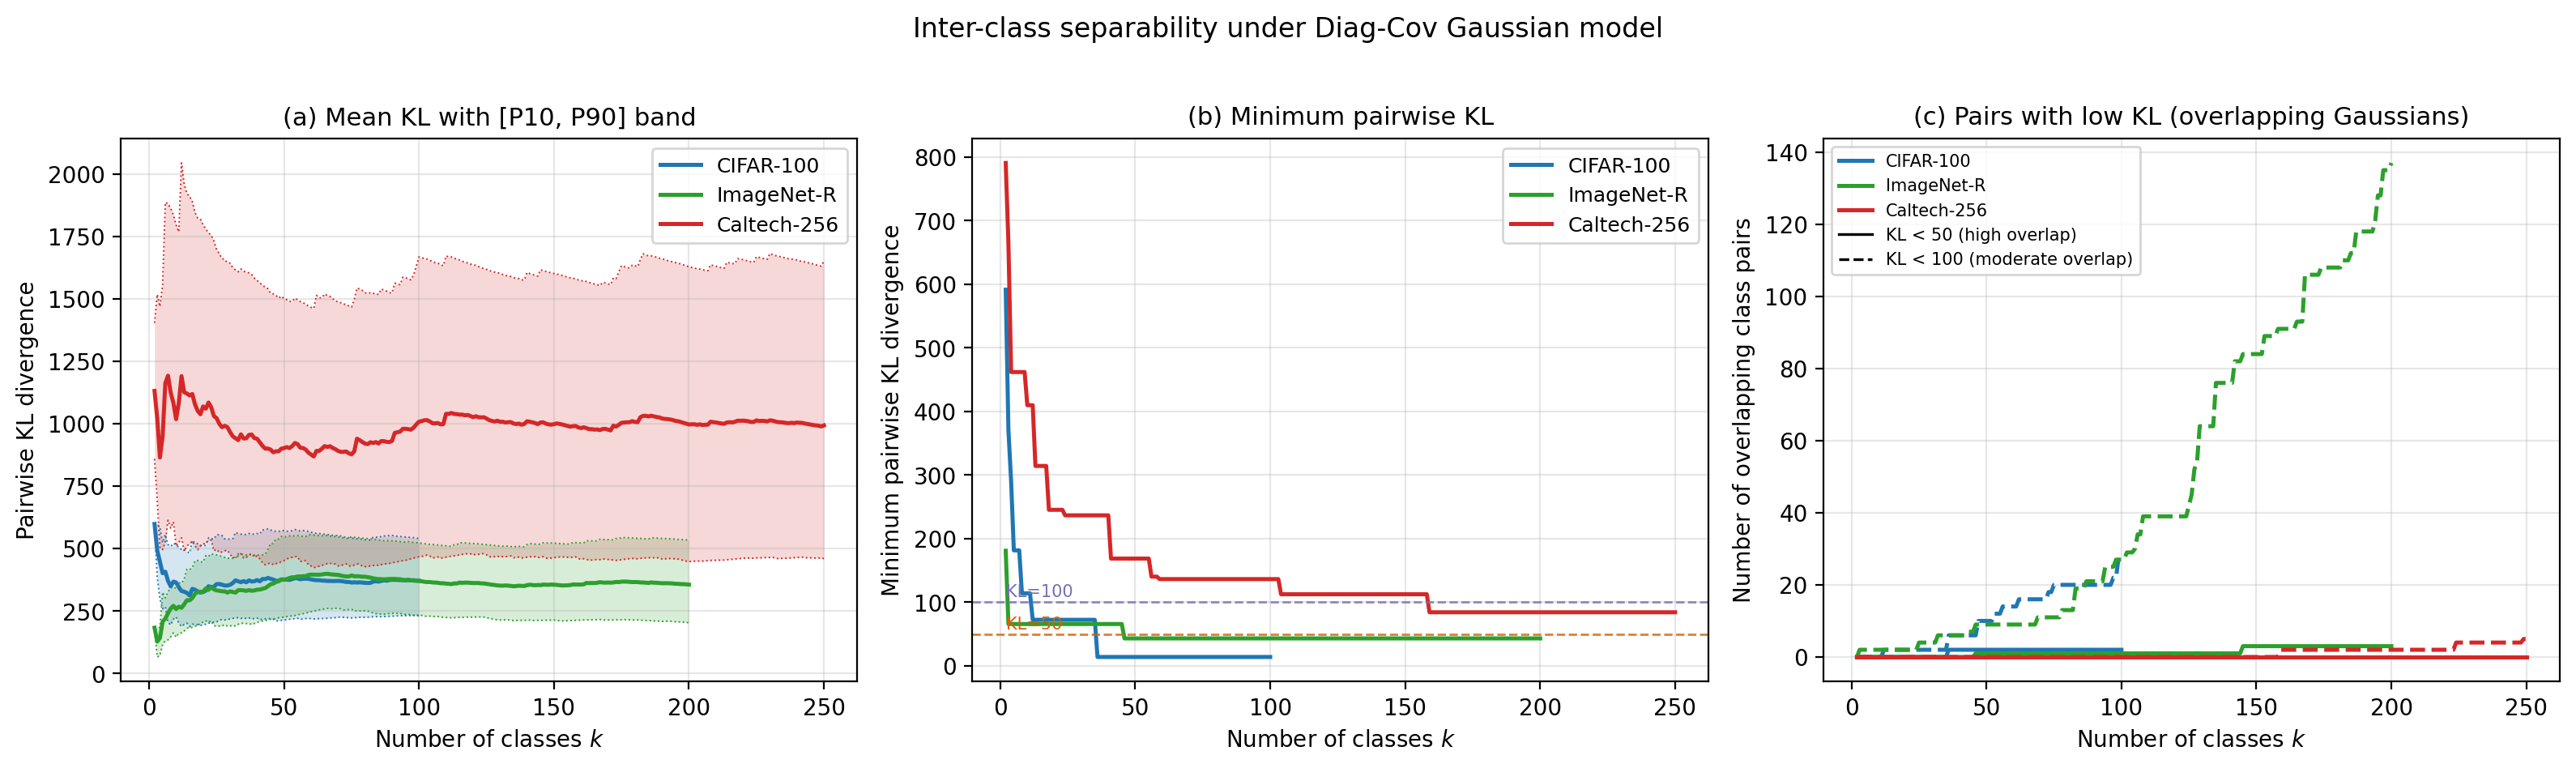
\includegraphics[width=0.99\linewidth]{imagenes/results/kl_divergence.png}
	\caption{Inter-class separability under the Diag-Cov Gaussian model as a function of the number of classes $k$. \textbf{(a)} Mean pairwise KL with $[\mathrm{P}_{10}, \mathrm{P}_{90}]$ shaded band. \textbf{(b)} Minimum pairwise KL: dashed lines mark KL~$=50$ and KL~$=100$. \textbf{(c)} Count of pairs below each overlap threshold. Over $99.7\,\%$ of all pairs remain well-separated (KL~$>100$) on every benchmark; the classifier's challenge is concentrated in the small tail of near-overlapping pairs.}
	\label{fig:kl_divergence}
\end{figure}

\section{Gaussianity Tests}
\label{sec:gaussianity_results_combined}

\subsection{Marginal Gaussianity}
\label{sec:gaussianity_results}
\phantomsection\label{sec:feature_space_diagnostics}

\begin{table}[htb]
	\centering
	\caption{Per-dimension Gaussianity statistics computed over all (class, coordinate) pairs of the frozen DINOv2 embeddings (raw, i.e.\ taken directly from the backbone). The columns $|\!\text{Skew}|_\mu$ and $|\!\text{Kurt}|_\mu$ are the mean absolute values; $\mathbb{P}[\cdot]$ denotes the empirical fraction of dimensions that satisfy each cut-off.}
	\label{tab:gaussianity_stats}
	\scriptsize
	\setlength{\tabcolsep}{4pt}
	\begin{tabular}{lcccccccc}
		\toprule
		\textbf{Dataset} & \textbf{n} & \textbf{Skew}$_\mu$ & $|\!\text{Skew}|_\mu$ & \textbf{Skew}$_\sigma$ & $\mathbb{P}[|\text{Skew}|{<}0.5]$ & \textbf{Kurt}$_\mu$ & $|\!\text{Kurt}|_\mu$ & $\mathbb{P}[|\text{Kurt}|{<}1]$ \\
		\midrule
		CIFAR-100         & 76\,800  & $-0.001$ & $0.181$ & $0.236$ & $0.961$ & $0.078$ & $0.264$ & $0.982$ \\
		ImageNet-R        & 153\,600 & $-0.002$ & $0.269$ & $0.348$ & $0.859$ & $0.115$ & $0.432$ & $0.924$ \\
		Caltech-256       & 192\,000 & $-0.001$ & $0.360$ & $0.472$ & $0.747$ & $0.402$ & $0.659$ & $0.822$ \\
		\bottomrule
	\end{tabular}
\end{table}

Table~\ref{tab:gaussianity_stats} reports the aggregate per-dimension Gaussianity statistics on each benchmark. The mean skewness is essentially zero on all three datasets ($|\text{Skew}_\mu|\le 0.002$), so the empirical mean is a faithful estimate of the class prototype and the assumption that the asymmetries are equally distributed between left and right tails is empirically supported. The dispersion of both moments, however, scales with the difficulty of the benchmark: the fraction of dimensions that satisfy $|\text{Skew}|<0.5$ drops from $96.1\,\%$ on CIFAR-100 to $85.9\,\%$ on ImageNet-R and $74.7\,\%$ on Caltech-256, while the mean absolute excess kurtosis rises from $0.26$ to $0.43$ and $0.66$, respectively. Figures~\ref{fig:skewness_histograms} and~\ref{fig:kurtosis_histograms} visualise the full empirical distributions: the histograms are sharply peaked around zero on CIFAR-100, mildly broadened on ImageNet-R and visibly heavier-tailed on Caltech-256, in agreement with the numerical summaries in the table.

\begin{figure}[htb]
	\centering
	\subfigure[CIFAR-100]{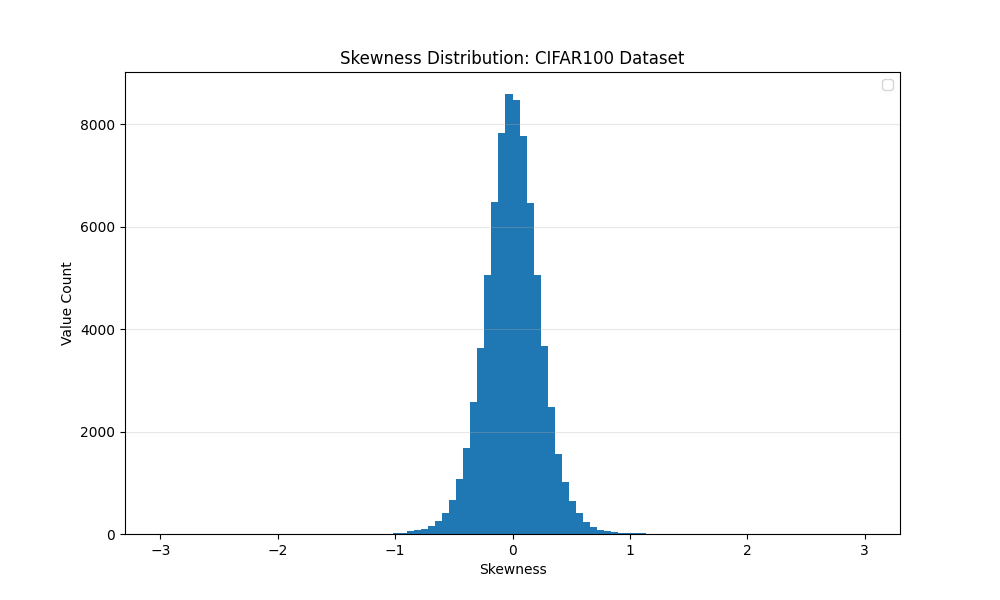
\includegraphics[width=0.32\linewidth]{imagenes/results/skewness_raw_cifar100.png}}
	\subfigure[ImageNet-R]{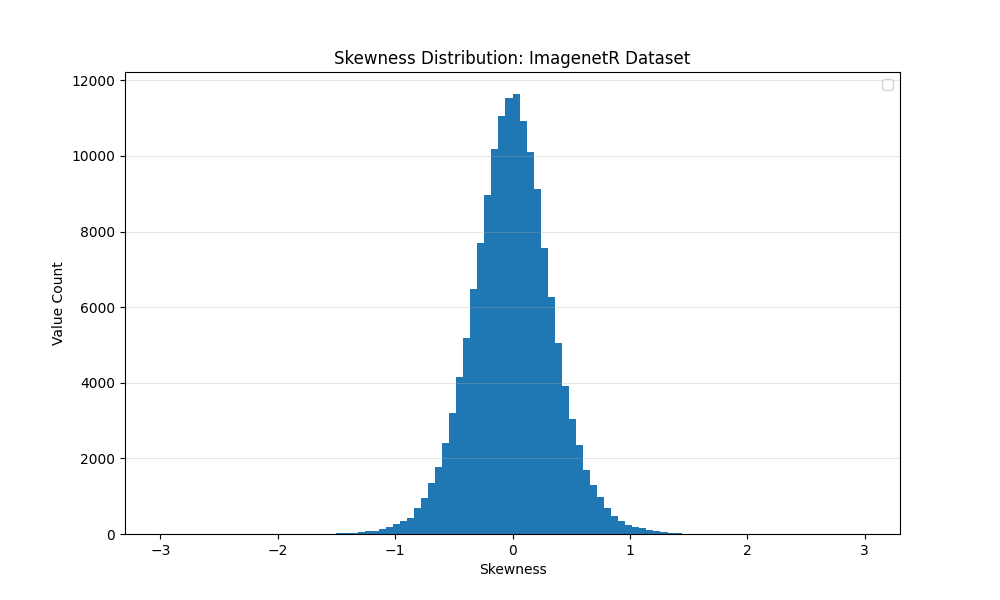
\includegraphics[width=0.32\linewidth]{imagenes/results/skewness_raw_imagenetR.png}}
	\subfigure[Caltech-256]{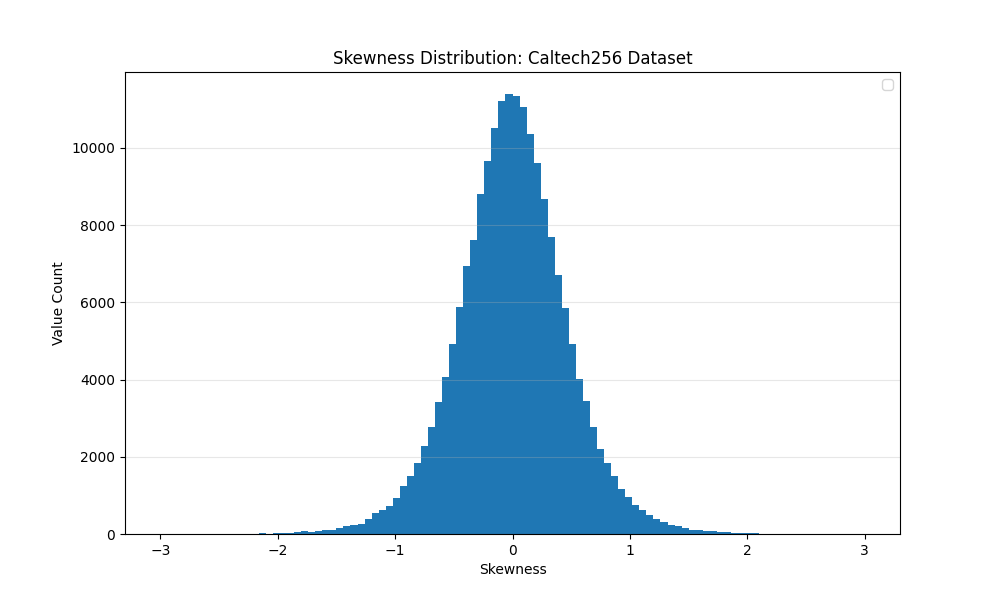
\includegraphics[width=0.32\linewidth]{imagenes/results/skewness_raw_caltech256.png}}
	\caption{Empirical skewness distribution over the $d \times C$ (class, coordinate) pairs of the DINOv2 embeddings.}
	\label{fig:skewness_histograms}
\end{figure}

\begin{figure}[htb]
	\centering
	\subfigure[CIFAR-100]{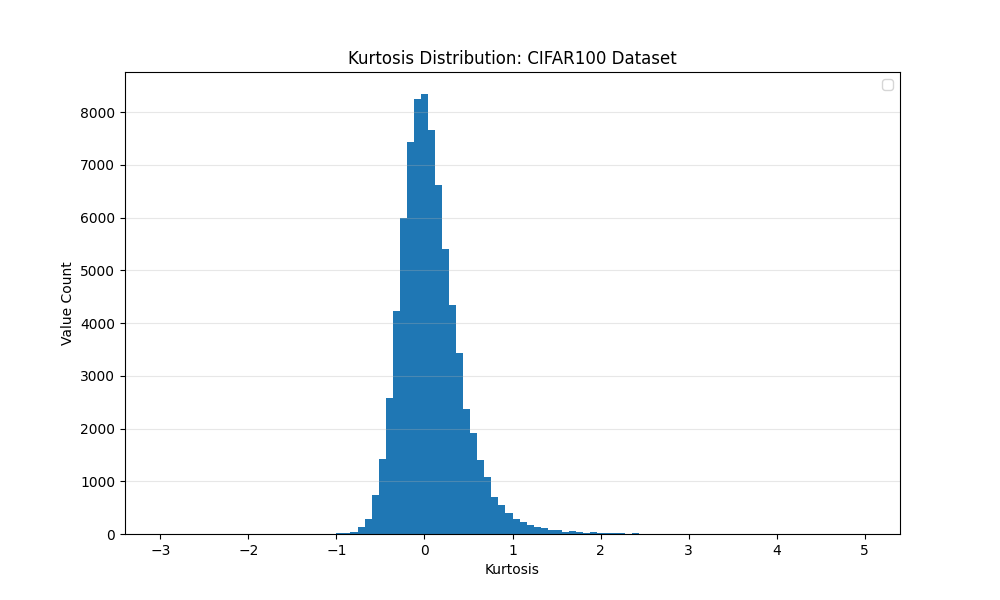
\includegraphics[width=0.32\linewidth]{imagenes/results/kurtosis_raw_cifar100.png}}
	\subfigure[ImageNet-R]{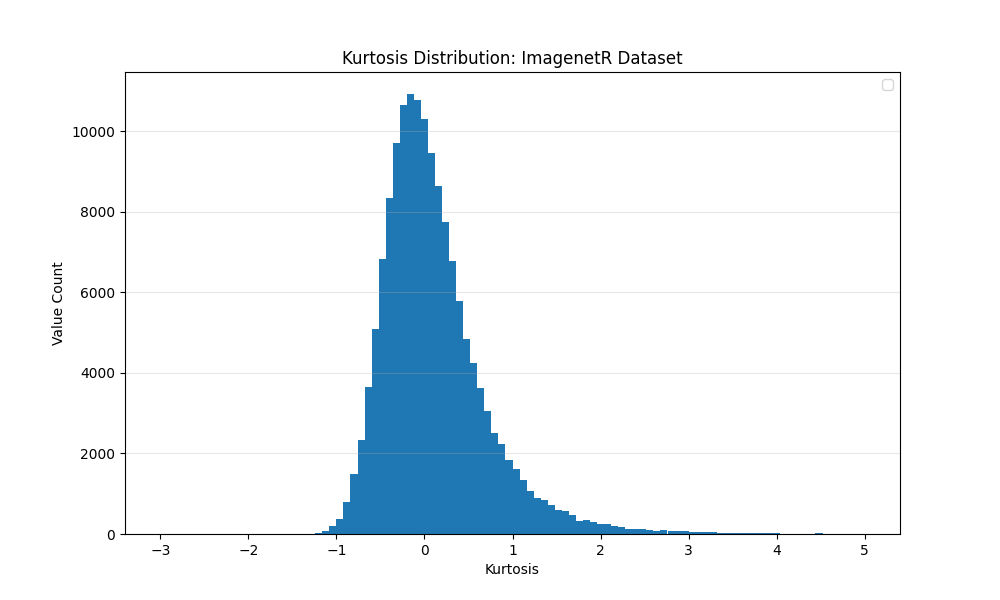
\includegraphics[width=0.32\linewidth]{imagenes/results/kurtosis_raw_imagenetR.png}}
	\subfigure[Caltech-256]{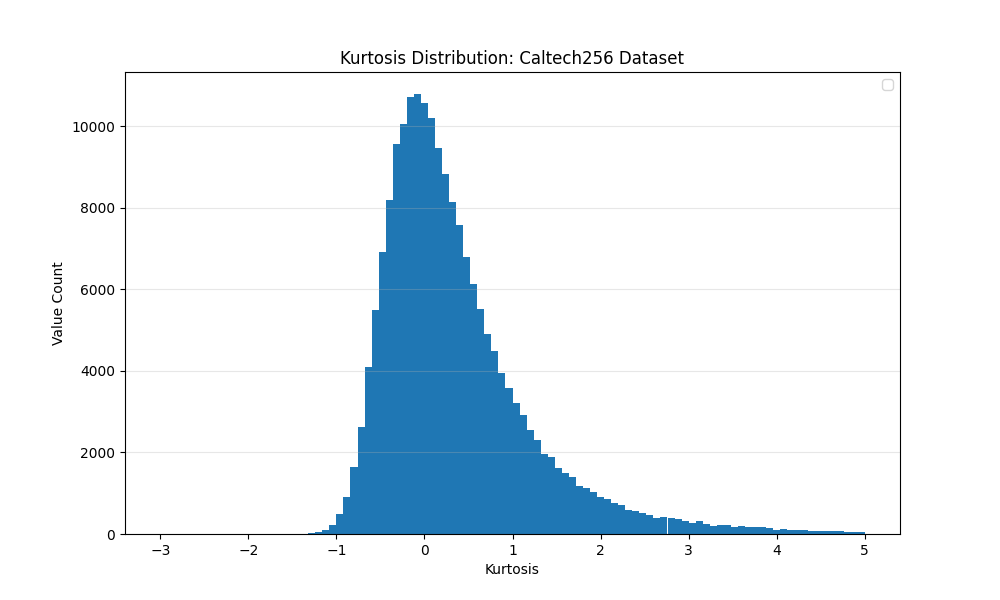
\includegraphics[width=0.32\linewidth]{imagenes/results/kurtosis_raw_caltech256.png}}
	\caption{Empirical excess-kurtosis distribution over the $d \times C$ (class, coordinate) pairs of the DINOv2 embeddings.}
	\label{fig:kurtosis_histograms}
\end{figure}

\begin{table}[htb]
	\centering
	\caption{Per-feature normality tests on the 80\,\% training split. \emph{normaltest} is the D'Agostino--Pearson composite test at $\alpha=0.05$ (H$_0$: the dimension is normally distributed); \emph{relaxed} is the joint criterion $|\mathrm{Skew}|<1$ \textbf{and} $|\mathrm{Kurt}|<1$; \emph{both} denotes pairs passing both. The median $p$-value is computed across all $(class, dimension)$ pairs.}
	\label{tab:gaussianity_normaltest}
	\scriptsize
	\setlength{\tabcolsep}{4pt}
	\begin{tabular}{lcccc}
		\toprule
		\textbf{Dataset} & \textbf{normaltest (\%)} & \textbf{relaxed (\%)} & \textbf{both (\%)} & \textbf{median $p$-value} \\
		\midrule
		CIFAR-100   & $70.0$ & $97.8$ & $70.0$ & $0.194$ \\
		ImageNet-R  & $80.8$ & $91.6$ & $79.7$ & $0.317$ \\
		Caltech-256 & $73.4$ & $82.3$ & $71.3$ & $0.244$ \\
		\bottomrule
	\end{tabular}
\end{table}

Two complementary per-feature normality assessments are reported in Table~\ref{tab:gaussianity_normaltest}.
The D'Agostino--Pearson normaltest at $\alpha=0.05$ provides the strictest formal criterion; it combines standardised skewness and kurtosis into a $\chi^2_2$ statistic and is therefore more sensitive than inspecting either moment alone.
The relaxed criterion---$|\mathrm{Skew}|<1$ \emph{and} $|\mathrm{Kurt}|<1$ simultaneously---is a lenient but transparent indicator of near-Gaussianity.
With training splits of $\bar{n}_c\approx400$, $120$ and $90$ samples per class for CIFAR-100, ImageNet-R and Caltech-256 respectively, even minor deviations from perfect normality are detectable, so the normaltest is conservative.
Nevertheless, $70$--$81\,\%$ of all (class, dimension) pairs pass the strict test, and the median $p$-value lies well above $0.05$ on every benchmark.
The relaxed criterion confirms that $82$--$98\,\%$ of pairs are near-Gaussian in both shape moments simultaneously.
Together with Table~\ref{tab:gaussianity_stats}, these results consistently support the marginal-Gaussianity assumption underlying the Diag-Cov classifier.

\subsection{Multivariate Gaussianity}
\label{sec:mv_gaussianity_results}

Table~\ref{tab:gaussianity_mv_kl} breaks down the multivariate Gaussianity assessment at the per-class level. For each class individually, the KL divergence between the empirical Diag-Cov squared Mahalanobis distance distribution and the theoretical $\chi^2_{768}$ reference is computed; this score measures how closely the class-conditional feature distribution conforms to the diagonal Gaussian assumption in the full $d=768$ dimensional space. Classes are then grouped into three departure bands: \emph{low} (KL~$<5$, approximately Gaussian), \emph{moderate} ($5 \le \text{KL} < 10$), and \emph{high} (KL~$\ge 10$, substantial departure).

\begin{table}[htb]
	\centering
	\caption{Per-class multivariate Gaussianity. The KL divergence $\mathrm{KL}(p_{\mathrm{emp}}\,\|\,\chi^2_{768})$ is computed for each class individually from its Diag-Cov squared Mahalanobis distances. \emph{Low} denotes KL~$<5$ (approximately Gaussian), \emph{Mod.}\ denotes $5 \le \mathrm{KL} < 10$, and \emph{High} denotes KL~$\ge 10$ (substantial departure). $\bar{n}_c$ is the median training samples per class.}
	\label{tab:gaussianity_mv_kl}
	\scriptsize
	\setlength{\tabcolsep}{6pt}
	\begin{tabular}{lcccccc}
		\toprule
		\textbf{Dataset} & $C$ & $\bar{n}_c$ & \textbf{KL mean} & \textbf{Low (\%)} & \textbf{Mod.\ (\%)} & \textbf{High (\%)} \\
		&  &  &  & \footnotesize{KL $< 5$} & \footnotesize{$5 \le$ KL $< 10$} & \footnotesize{KL $\ge 10$} \\
		\midrule
		Split CIFAR-100   & 100 & 400 & $5.98$  & $39.0$ & $53.0$ & $\phantom{0}8.0$ \\
		Split ImageNet-R  & 200 & 110 & $8.11$  & $16.5$ & $51.5$ & $32.0$ \\
		Split Caltech-256 & 250 &  80 & $10.38$ & $\phantom{0}4.4$ & $32.8$ & $62.8$ \\
		\bottomrule
	\end{tabular}
\end{table}

\section{Confidence and Calibration Metrics}
\label{sec:calibration_results_section}

Table~\ref{tab:calibration_metrics} reports six metrics that characterise the probabilistic behaviour of the Gaussian classifier: the final-task accuracy ($A_T$ in \%), the Expected Calibration Error (ECE, \%), the Confidence on Errors (CoE), Total Confidence (TC), Probability Margin (PM), and the Predictive Entropy. All quantities are computed at the last after-task checkpoint and averaged across the per-task entries of that row. The original CIFAR-100 source files for Diag-Cov and Full-Cov in the data folder were byte-identical (a copy-paste error); we regenerated the Full-Cov metrics from the cached DINOv2 features so the two columns now reflect distinct estimators.

Two observations are worth noting for the Diag-Cov rows. First, TC and PM are systematically different: TC measures the raw top-1 probability while PM measures the \emph{margin} between the top-1 and top-2 probabilities. The gap between them ($\mathrm{TC}-\mathrm{PM} \approx 0.02$--$0.06$ depending on the dataset) represents the average probability mass placed on the runner-up class. On CIFAR-100, for instance, TC$=0.836$ but PM$=0.774$: the model is 83.6\% confident in its top choice, yet only 77.4\% more confident than its second choice, meaning the runner-up class retains roughly 6\% probability on average. This gap is largest on ImageNet-R and CIFAR-100---datasets with more visual ambiguity---and smallest on Caltech-256, where higher visual distinctiveness leaves little probability on the runner-up. Second, both TC and PM are substantially higher than the corresponding accuracy, confirming the overconfidence phenomenon discussed in Section~\ref{sec:method:highdimdim}.

\begin{table}[htbp]
	\centering
	\caption{Probabilistic calibration metrics for the Bayesian classifier at the last after-task checkpoint. Accuracy and ECE are in percentage points; CoE, TC, PM and Entropy are in $[0,1]$. PM (Probability Margin) is the average difference $p_{(1)}-p_{(2)}$ between the top-1 and top-2 softmax probabilities; TC is the average of $p_{(1)}$ alone. Lower is better for ECE and CoE; higher is better for Accuracy. CIFAR-100 Full was regenerated from the cached DINOv2 features because the original source file was a byte-identical copy of the Diag one.}
	\label{tab:calibration_metrics}
	\scriptsize
	\setlength{\tabcolsep}{3pt}
	\begin{tabular}{l|cc|cc|cc|cc}
		\toprule
		\textbf{Metric} & \multicolumn{2}{c|}{\textbf{CIFAR-100}} & \multicolumn{2}{c|}{\textbf{ImageNet-R}} & \multicolumn{2}{c|}{\textbf{Caltech-256}} & \multicolumn{2}{c}{\textbf{Joint}} \\
		                & Diag & Full & Diag & Full & Diag & Full & Diag & Full \\
		\midrule
		Accuracy (\%)        & 86.07 & 88.48 & 77.12 & 75.08 & 90.06 & 90.01 & 78.32 & 78.65 \\
		ECE (\%)             & 3.72  & 11.68 & 13.72 & 37.44 & 7.05  & 26.03 & 11.46 & 29.05 \\
		Confidence on Errors & 0.467 & 1.000 & 0.656 & 1.000 & 0.805 & 1.000 & 0.742 & 1.000 \\
		Total Confidence     & 0.836 & 1.000 & 0.883 & 1.000 & 0.974 & 1.000 & 0.931 & 1.000 \\
		Probability Margin   & 0.774 & 1.000 & 0.825 & 1.000 & 0.955 & 1.000 & 0.890 & 1.000 \\
		Predictive Entropy   & 0.614 & 0.000 & 0.365 & 0.000 & 0.067 & 0.000 & 0.207 & 0.000 \\
		\bottomrule
	\end{tabular}
\end{table}

A particularly striking result in Table~\ref{tab:calibration_metrics} is the Full-Cov column: the Confidence on Errors reaches $1.000$ on every benchmark, the Total Confidence is identically $1.000$, and the predictive entropy collapses to $0.000$. This is a direct consequence of the rank-deficient covariance estimation discussed in Section~\ref{sec:feature_space_diagnostics}: the Mahalanobis distances under the Full-Cov model are degenerate (collapsing to a spike at $\overline{n_c}-1$), making the log-likelihood of the nearest class astronomically larger than any other; the resulting softmax posterior is a hard one-hot assignment that is always maximally confident, regardless of whether the prediction is correct.
Figure~\ref{fig:coe_histograms} visualises the distribution of CoE values pooled from the full lower-triangular evaluation matrix.
Because the continual-learning protocol evaluates the model after each of the $T=10$ tasks on every task seen so far, each benchmark produces a $T\times T$ lower-triangular matrix whose $(t,s)$ entry is the CoE when evaluating on task $s$ after training on tasks $1,\ldots,t$ ($s \le t$).
The histogram therefore contains $T(T+1)/2 = 55$ data points per benchmark, and the $y$-axis counts how many of those 55 evaluation pairs fall in each CoE bin---it is not the number of tasks.
The Diag-Cov distributions are well-spread and shift rightward as benchmark difficulty increases (CIFAR-100 peak near $0.47$, ImageNet-R near $0.66$, Caltech-256 near $0.81$), reflecting that the classifier becomes more confidently wrong on harder datasets.
The Full-Cov distributions collapse to degenerate spikes at $\mathrm{CoE}=1.0$: all 55 evaluation pairs pile into a single bin, giving the high count visible in the figure, which confirms the rank-deficiency pathology described above.

\begin{figure}[htbp]
	\centering
	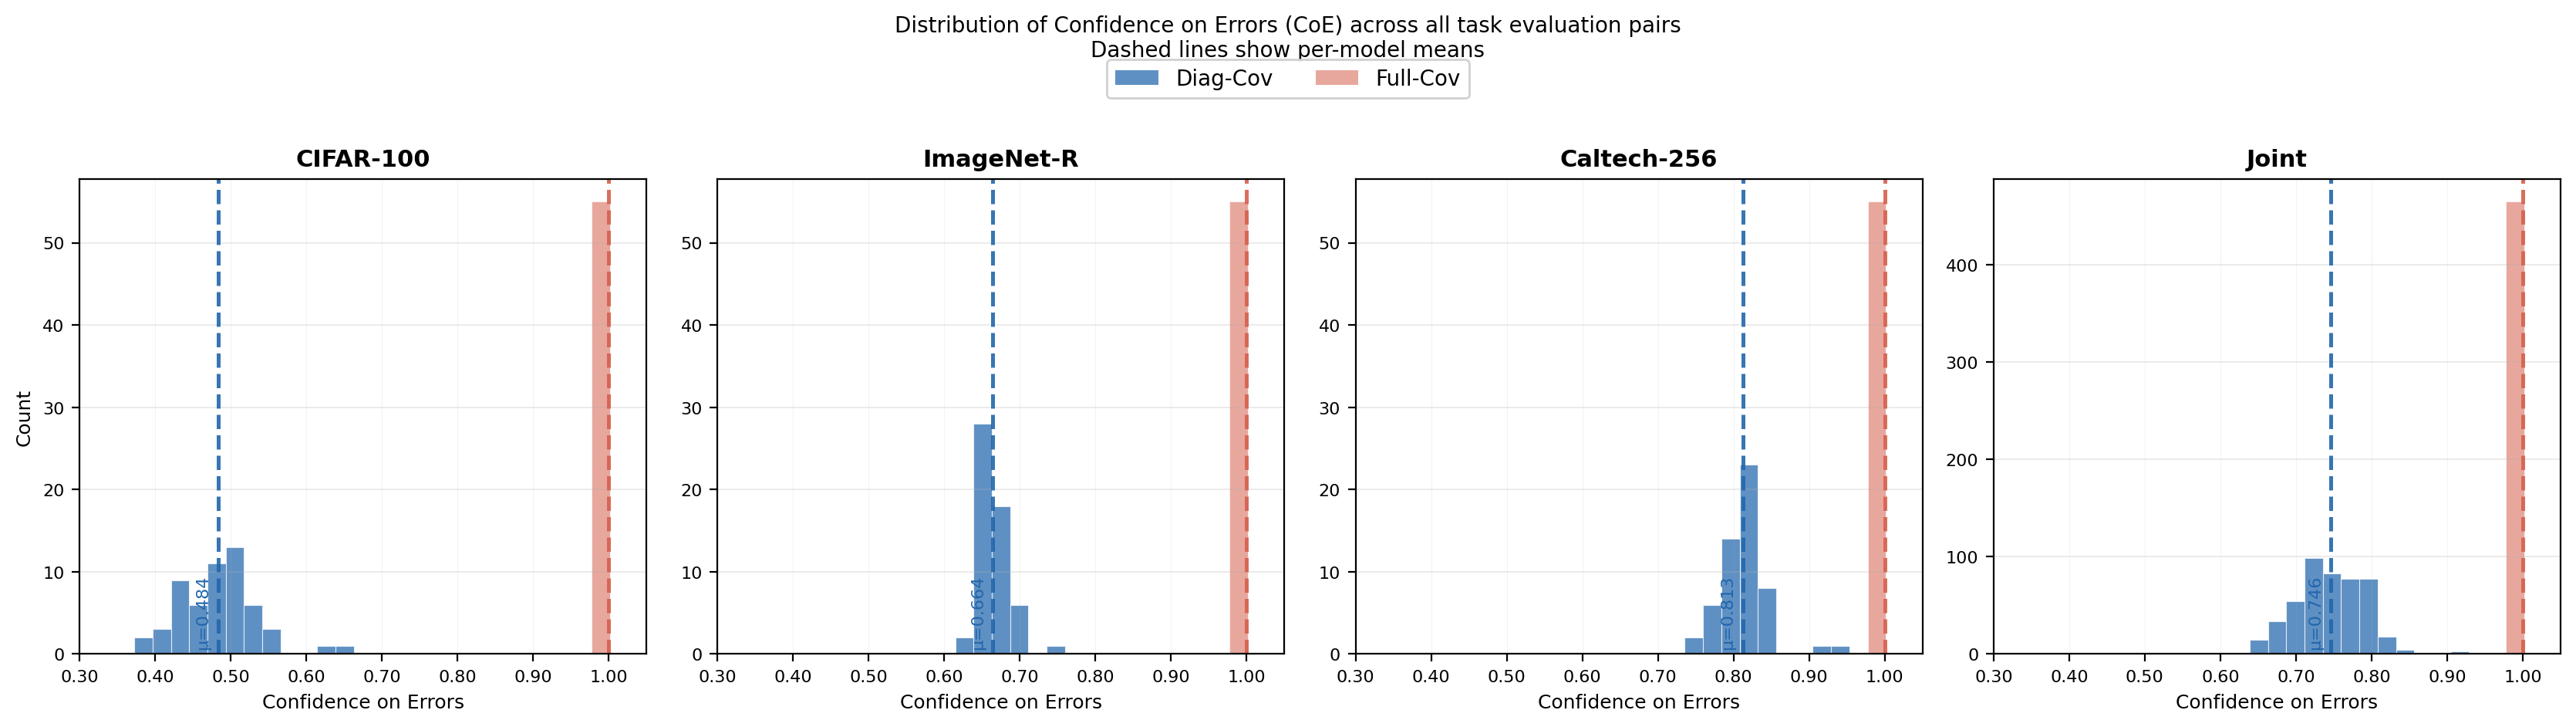
\includegraphics[width=0.97\linewidth]{imagenes/results/coe_histograms.png}
	\caption{Distribution of Confidence on Errors (CoE) over the $T(T+1)/2=55$ lower-triangular evaluation pairs per benchmark ($T=10$ tasks). The $y$-axis is the count of evaluation pairs falling in each CoE bin, not the number of tasks. Diag-Cov values are spread across $[0.3,\,1.0]$ and shift rightward with dataset difficulty; Full-Cov values collapse entirely to $\mathrm{CoE}=1.0$, yielding a degenerate spike whose height equals the total number of evaluation pairs.}
	\label{fig:coe_histograms}
\end{figure}

Figure~\ref{fig:coe_evolution} shows how the mean CoE evolves across successive training checkpoints. At checkpoint $t$, the mean is taken over the $t$ available lower-triangular entries of row $t$ (i.e.\ the CoE when evaluating on each of the $t$ tasks seen so far). For Diag-Cov the mean CoE rises gradually as more tasks accumulate---reflecting growing inter-class confusion---and the effect is strongest on Caltech-256, where intra-class visual variability is highest. For Full-Cov, CoE stays pinned at $1.0$ from the very first checkpoint.

\begin{figure}[htbp]
	\centering
	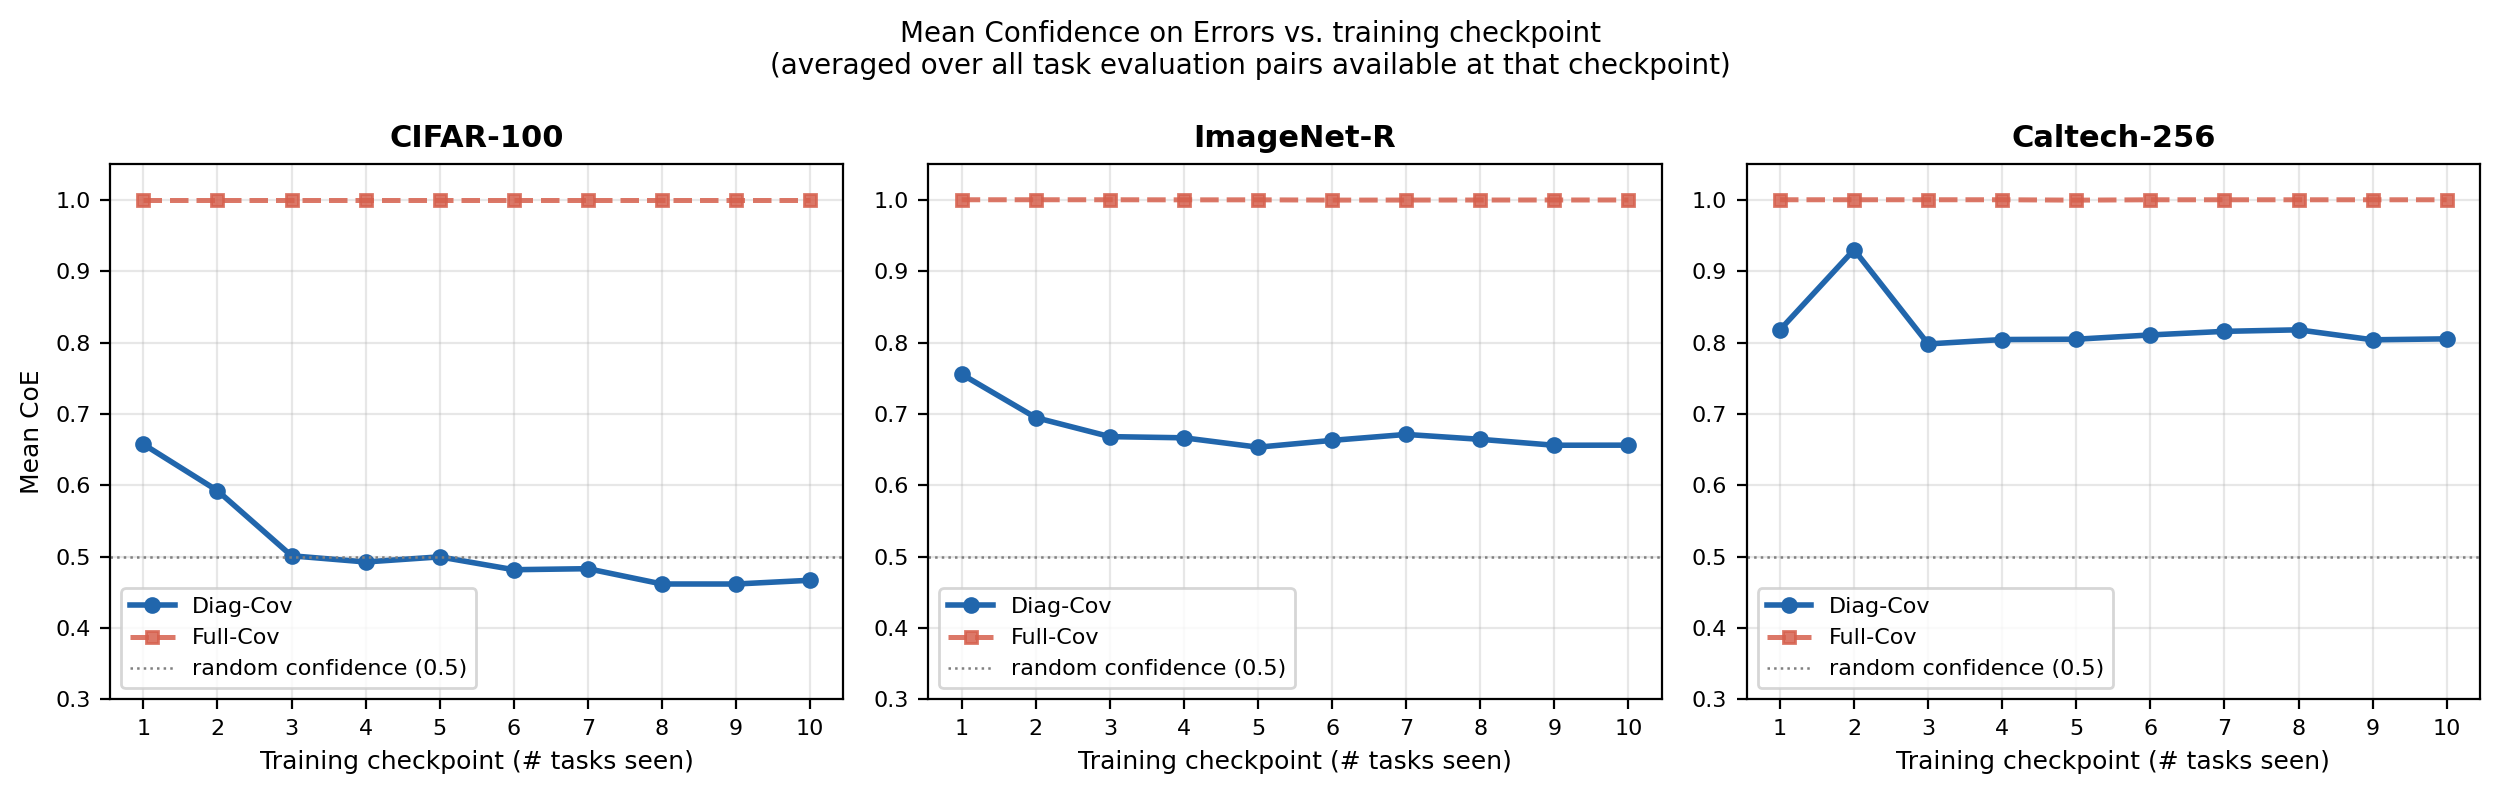
\includegraphics[width=0.97\linewidth]{imagenes/results/coe_evolution.png}
	\caption{Mean Confidence on Errors at each training checkpoint $t$, averaged over the $t$ lower-triangular evaluation pairs available at that checkpoint. Diag-Cov (solid) rises gradually as more tasks are added; Full-Cov (dashed) remains degenerate at $1.0$ throughout.}
	\label{fig:coe_evolution}
\end{figure}
